\documentclass[aspectratio=169,11pt]{beamer}

\usetheme{Madrid}
\usecolortheme{whale}
\setbeamertemplate{navigation symbols}{}
\setbeamertemplate{footline}[frame number]

\usepackage[utf8]{inputenc}
\usepackage[T1]{fontenc}
\usepackage{booktabs}
\usepackage{xcolor}
\usepackage{hyperref}
\usepackage{listings}
\usepackage{tikz}
\usetikzlibrary{shapes,arrows,positioning,calc,fit}

\lstset{
    basicstyle=\ttfamily\scriptsize,
    breaklines=true,
    frame=single,
    backgroundcolor=\color{gray!10},
    keywordstyle=\color{blue!70},
    commentstyle=\color{green!50!black},
    stringstyle=\color{red!60},
    showstringspaces=false,
    tabsize=2
}

\definecolor{stepbg}{RGB}{232,245,233}
\definecolor{stepborder}{RGB}{76,175,80}
\definecolor{warnbg}{RGB}{255,243,224}
\definecolor{warnborder}{RGB}{255,152,0}
\definecolor{aibg}{RGB}{243,229,245}
\definecolor{aiborder}{RGB}{156,39,176}
\definecolor{nodered}{RGB}{142,31,11}

\title[EECE5155 -- Hands-On 2]{Node-RED: IoT Automation \& Dashboards}
\subtitle{Hands-On Session 2: Build Logic Flows Without Hardware}
\author{Eduardo Baena}
\date{Wednesday, March 25, 2026}
\institute{Northeastern University\\EECE5155: Wireless Sensor Networks and IoT}

\begin{document}

\begin{frame}
    \titlepage
\end{frame}

%==============================================================================
\section{Context}
%==============================================================================

\begin{frame}{This Week: From Sensor to Dashboard}
    \begin{center}
    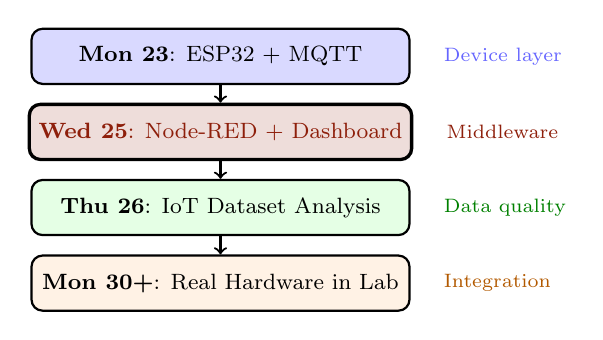
\begin{tikzpicture}[
        scale=0.8,
        every node/.style={font=\footnotesize},
        day/.style={draw, rounded corners, minimum width=4.8cm, minimum height=0.7cm, thick},
    ]
        \node[day, fill=blue!15] (mon) at (0,3) {\textbf{Mon 23}: ESP32 + MQTT};
        \node[day, fill=nodered!15, text=nodered, very thick] (wed) at (0,1.8) {\textbf{Wed 25}: Node-RED + Dashboard};
        \node[day, fill=green!10] (thu) at (0,0.6) {\textbf{Thu 26}: IoT Dataset Analysis};
        \node[day, fill=orange!10] (sat) at (0,-0.6) {\textbf{Mon 30+}: Real Hardware in Lab};

        \draw[->,thick] (mon) -- (wed);
        \draw[->,thick] (wed) -- (thu);
        \draw[->,thick] (thu) -- (sat);

        \node[font=\scriptsize, right, text=blue!60] at (mon.east) [xshift=0.3cm] {Device layer};
        \node[font=\scriptsize, right, text=nodered] at (wed.east) [xshift=0.3cm] {Middleware};
        \node[font=\scriptsize, right, text=green!50!black] at (thu.east) [xshift=0.3cm] {Data quality};
        \node[font=\scriptsize, right, text=orange!70!black] at (sat.east) [xshift=0.3cm] {Integration};
    \end{tikzpicture}
    \end{center}

    \vspace{0.2cm}
    \textbf{Monday recap:} We wrote ESP32 firmware that reads a DHT22 sensor and publishes JSON over MQTT to \texttt{broker.hivemq.com}. That data is flowing right now.

    \vspace{0.15cm}
    \textbf{Today's question:} What happens to the data after the broker receives it? Right now: nothing. We build the middleware that subscribes, parses, visualizes, and alerts.
\end{frame}

%==============================================================================
\section{What Is Node-RED?}
%==============================================================================

\begin{frame}[shrink=5]{Node-RED: Visual Programming for IoT}
    \begin{columns}
        \column{0.55\textwidth}
        \textbf{What it is:}
        \begin{itemize}
            \item Open-source flow-based programming tool
            \item Built on Node.js, browser-based editor
            \item Drag-and-drop nodes to create IoT logic
            \item Used in production by IBM, Bosch, Siemens
        \end{itemize}

        \vspace{0.15cm}
        \textbf{Why it matters for your project:}
        \begin{itemize}
            \item Process incoming MQTT data
            \item Apply rules and thresholds (alerts)
            \item Transform and route data
            \item Build real-time dashboards
            \item No backend code required
        \end{itemize}

        \column{0.45\textwidth}
        \textbf{How it connects:}

        \vspace{0.1cm}
        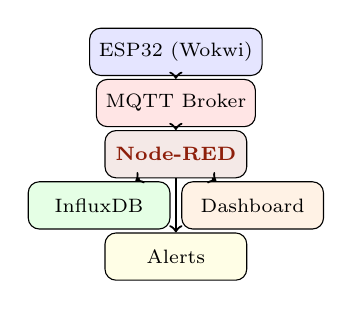
\begin{tikzpicture}[
            scale=0.65,
            every node/.style={font=\scriptsize},
            box/.style={draw, rounded corners, minimum width=1.8cm, minimum height=0.6cm, fill=white},
        ]
            \node[box, fill=blue!10] (esp) at (0,3) {ESP32 (Wokwi)};
            \node[box, fill=red!10] (mqtt) at (0,2) {MQTT Broker};
            \node[box, fill=nodered!10, text=nodered] (nr) at (0,1) {\textbf{Node-RED}};
            \node[box, fill=green!10] (db) at (-1.5,0) {InfluxDB};
            \node[box, fill=orange!10] (dash) at (1.5,0) {Dashboard};
            \node[box, fill=yellow!10] (alert) at (0,-1) {Alerts};

            \draw[->,thick] (esp) -- (mqtt);
            \draw[->,thick] (mqtt) -- (nr);
            \draw[->,thick] (nr) -- (db);
            \draw[->,thick] (nr) -- (dash);
            \draw[->,thick] (nr) -- (alert);
        \end{tikzpicture}

        \vspace{0.1cm}
        \fcolorbox{aiborder}{aibg}{
        \begin{minipage}{0.85\textwidth}
            \tiny
            \textbf{vs Cloud hands-on:} You built MQTT $\rightarrow$ InfluxDB $\rightarrow$ Grafana with Docker. Node-RED adds \textbf{logic, automation, and rapid prototyping}.
        \end{minipage}
        }
    \end{columns}
\end{frame}

%==============================================================================
\section{Flow-Based Programming}
%==============================================================================

\begin{frame}[shrink=5]{Flow-Based Programming: The Paradigm Behind Node-RED}
    \begin{columns}
        \column{0.55\textwidth}
        \textbf{Origin:}
        \begin{itemize}
            \item Invented by J. Paul Morrison at IBM (1970s)
            \item Programs as networks of ``black box'' processes
            \item Data flows between processes via connections
            \item Each process: independent, reusable, testable
        \end{itemize}

        \vspace{0.15cm}
        \textbf{Node-RED history:}
        \begin{itemize}
            \item Created at IBM Emerging Technology (2013)
            \item Originally for wiring IoT hardware APIs
            \item Open-sourced 2013, JS Foundation 2016
            \item OpenJS Foundation project since 2019
            \item 5,000+ community nodes available
        \end{itemize}

        \column{0.45\textwidth}
        \textbf{Flow-based vs imperative:}

        \vspace{0.1cm}
        \fcolorbox{stepborder}{stepbg}{
        \begin{minipage}{0.9\textwidth}
            \vspace{0.1cm}
            \scriptsize
            \textbf{Imperative (Python):}\\
            Subscribe $\rightarrow$ parse $\rightarrow$ check threshold $\rightarrow$ if true, alert $\rightarrow$ store $\rightarrow$ dashboard\\
            \textit{300+ lines, error handling, server setup}

            \vspace{0.15cm}
            \textbf{Flow-based (Node-RED):}\\
            Wire 6 nodes, each encapsulates one responsibility.\\
            \textit{Visible dataflow. Modify without rewriting.}
            \vspace{0.1cm}
        \end{minipage}
        }

        \vspace{0.15cm}
        \fcolorbox{aiborder}{aibg}{
        \begin{minipage}{0.9\textwidth}
            \tiny
            \textbf{Key insight:} Flow-based programming separates \textit{what} a component does from \textit{how} components connect. You can swap a ``store to InfluxDB'' node for ``store to PostgreSQL'' without touching any other logic.
        \end{minipage}
        }
    \end{columns}
\end{frame}

%==============================================================================
\section{IoT Pipeline Architecture}
%==============================================================================

\begin{frame}[shrink=10]{Where Node-RED Fits: End-to-End IoT Architecture}
    \begin{columns}
        \column{0.5\textwidth}
        \begin{center}
        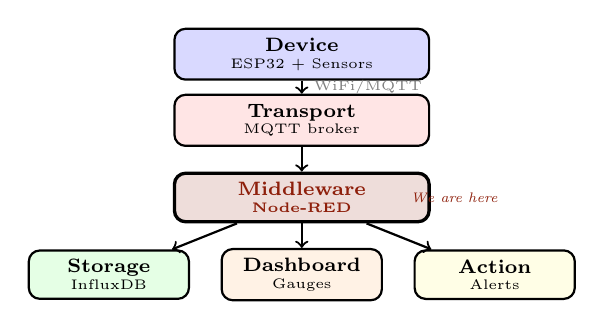
\begin{tikzpicture}[
            scale=0.7,
            every node/.style={font=\tiny},
            top/.style={draw, rounded corners, minimum height=0.55cm, thick, text width=3cm, align=center},
            bot/.style={draw, rounded corners, minimum height=0.55cm, thick, text width=1.8cm, align=center},
        ]
            \node[top, fill=blue!15] (device) at (0,4) {\scriptsize\textbf{Device}\\\tiny ESP32 + Sensors};
            \node[top, fill=red!10] (transport) at (0,2.8) {\scriptsize\textbf{Transport}\\\tiny MQTT broker};
            \node[top, fill=nodered!15, text=nodered, very thick] (middleware) at (0,1.4) {\scriptsize\textbf{Middleware}\\\tiny\textbf{Node-RED}};
            \node[bot, fill=green!10] (storage) at (-3.5,0) {\scriptsize\textbf{Storage}\\\tiny InfluxDB};
            \node[bot, fill=orange!10] (viz) at (0,0) {\scriptsize\textbf{Dashboard}\\\tiny Gauges};
            \node[bot, fill=yellow!10] (action) at (3.5,0) {\scriptsize\textbf{Action}\\\tiny Alerts};

            \draw[->,thick] (device) -- (transport);
            \draw[->,thick] (transport) -- (middleware);
            \draw[->,thick] (middleware) -- (storage);
            \draw[->,thick] (middleware) -- (viz);
            \draw[->,thick] (middleware) -- (action);

            \node[font=\tiny, text=gray] at (1.2,3.4) {WiFi/MQTT};
            \node[font=\tiny, text=nodered, right] at (1.8,1.4) {\textit{We are here}};
        \end{tikzpicture}
        \end{center}

        \column{0.5\textwidth}
        \textbf{What Node-RED does as middleware:}
        \begin{itemize}
            \item \textbf{Parse + transform}: JSON $\rightarrow$ extract fields, convert units
            \item \textbf{Route data}: to databases, dashboards, APIs
            \item \textbf{Threshold logic}: alert when values cross limits
            \item \textbf{Actuation}: send commands back to devices (relay on/off, valve open/close)
            \item \textbf{Data fusion}: combine multiple sensor streams into derived metrics
            \item \textbf{Protocol bridge}: MQTT $\leftrightarrow$ HTTP $\leftrightarrow$ Modbus $\leftrightarrow$ OPC-UA
        \end{itemize}

        \vspace{0.1cm}
        \fcolorbox{stepborder}{stepbg}{
        \begin{minipage}{0.95\textwidth}
            \tiny
            \textbf{Industry use:} Node-RED is deployed by IBM, Bosch, Siemens, and Hitachi for production monitoring, equipment control, and energy management (2023 Node-RED survey: 40\% manufacturing use).
        \end{minipage}
        }
    \end{columns}

    \vspace{0.1cm}
    {\small \textbf{Monday}: Device $\rightarrow$ Transport \quad\quad \textbf{Today}: Transport $\rightarrow$ Middleware $\rightarrow$ Dashboard + Alerts}
\end{frame}

\begin{frame}[fragile,shrink=5]{The Node-RED Interface}
    \begin{columns}
        \column{0.55\textwidth}
        \textbf{Four areas of the editor:}
        \begin{enumerate}
            \item \textbf{Node Palette} (left): all available nodes, categorized
            \item \textbf{Flow Canvas} (center): drag, drop, wire nodes
            \item \textbf{Info/Debug Panel} (right): node docs + debug output
            \item \textbf{Deploy Button} (top right): push changes live
        \end{enumerate}

        \vspace{0.15cm}
        \textbf{Core concepts:}
        \begin{itemize}
            \item \textbf{Node}: one operation (input, process, or output)
            \item \textbf{Wire}: data connection between nodes
            \item \textbf{Flow}: a tab containing a group of connected nodes
            \item \textbf{msg.payload}: the data object passed between nodes
        \end{itemize}

        \column{0.45\textwidth}
        \textbf{Message structure:}
        \begin{lstlisting}[basicstyle=\ttfamily\tiny]
// Every node receives a "msg" object
{
  "topic": "eece5155/.../sensors",
  "payload": {
    "temp": 23.5,
    "hum": 65.2
  },
  "_msgid": "abc123"
}
// Your job: transform msg.payload
// and pass it to the next node
        \end{lstlisting}

        \vspace{0.1cm}
        \fcolorbox{warnborder}{warnbg}{
        \begin{minipage}{0.9\textwidth}
            \tiny
            \textbf{Rule:} Every function node must end with \texttt{return msg;} or the message stops. This is the most common beginner mistake.
        \end{minipage}
        }
    \end{columns}
\end{frame}

%==============================================================================
\section{Setup}
%==============================================================================

\begin{frame}[fragile]{Step 0: Install Node-RED (5 min)}
    \textbf{Option A: npm (recommended)}
    \begin{lstlisting}[language=bash]
# Install Node-RED globally
npm install -g --unsafe-perm node-red

# Start Node-RED
node-red
    \end{lstlisting}

    \textbf{Option B: Docker (if you have Docker from cloud hands-on)}
    \begin{lstlisting}[language=bash]
docker run -it -p 1880:1880 --name nodered nodered/node-red
    \end{lstlisting}

    \vspace{0.2cm}
    \begin{enumerate}
        \item Open \url{http://localhost:1880} in your browser
        \item You should see the Node-RED flow editor
        \item Install dashboard nodes: Menu $\rightarrow$ Manage Palette $\rightarrow$ Install $\rightarrow$ search \texttt{@flowfuse/node-red-dashboard}
    \end{enumerate}

    \vspace{0.1cm}
    \fcolorbox{stepborder}{stepbg}{
    \begin{minipage}{0.95\textwidth}
        \small
        \textbf{Prerequisite:} Node.js $\geq$ 18. Check with \texttt{node --version}. Install from \url{https://nodejs.org/} if needed.
    \end{minipage}
    }
\end{frame}

%==============================================================================
\section{Exercise 1: MQTT Receiver}
%==============================================================================

\begin{frame}[fragile,shrink=15]{Exercise 1: Receive MQTT Data (15 min)}
    \textbf{Build a flow that receives data from your Wokwi ESP32:}

    \vspace{0.15cm}
    \begin{columns}
        \column{0.6\textwidth}
        \textbf{Steps:}
        \begin{enumerate}
            \item Drag an \textbf{mqtt in} node onto the canvas
            \item Double-click to configure:
            \begin{itemize}
                \item Server: \texttt{broker.hivemq.com:1883}
                \item Topic: \texttt{eece5155/YOUR\_NAME/sensors}
            \end{itemize}
            \item Drag a \textbf{debug} node and connect them
            \item Click \textbf{Deploy} (top right)
            \item Run your Wokwi project from Monday
            \item Check the debug panel (right sidebar)
        \end{enumerate}

        \vspace{0.1cm}
        \textbf{No Wokwi running?} Use the MQTT simulator:
        \begin{lstlisting}[language=bash,basicstyle=\ttfamily\tiny]
pip install paho-mqtt
python3 -c "
import paho.mqtt.client as mqtt, json, time, random
c = mqtt.Client(mqtt.CallbackAPIVersion.VERSION2)
c.connect('broker.hivemq.com', 1883)
c.loop_start()
while True:
    d = {'temp': round(random.uniform(18,30),1),
         'hum': round(random.uniform(40,80),1)}
    c.publish('eece5155/YOUR_NAME/sensors', json.dumps(d))
    time.sleep(5)"
        \end{lstlisting}

        \column{0.4\textwidth}
        \textbf{Node-RED flow:}

        \vspace{0.1cm}
        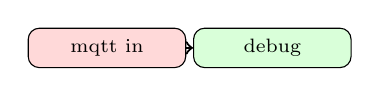
\begin{tikzpicture}[
            scale=0.7,
            every node/.style={font=\scriptsize},
            node/.style={draw, rounded corners, minimum width=2cm, minimum height=0.5cm},
        ]
            \node[node, fill=red!15] (mqtt) at (0,0) {mqtt in};
            \node[node, fill=green!15] (debug) at (3,0) {debug};
            \draw[->,thick] (mqtt) -- (debug);
        \end{tikzpicture}

        \vspace{0.2cm}
        \fcolorbox{warnborder}{warnbg}{
        \begin{minipage}{0.85\textwidth}
            \vspace{0.05cm}
            \tiny
            \textbf{Verify:} You see JSON messages in the debug panel every 10 seconds. If not, check topic name matches exactly.
            \vspace{0.05cm}
        \end{minipage}
        }
    \end{columns}
\end{frame}

%==============================================================================
\section{Exercise 2: Parse + Dashboard}
%==============================================================================

\begin{frame}[fragile,shrink=5]{Exercise 2a: Parse JSON (5 min)}
    \textbf{The MQTT message is a string. We need to parse it into an object.}

    \vspace{0.15cm}
    \begin{columns}
        \column{0.55\textwidth}
        \textbf{Before parsing (raw string):}
        \begin{lstlisting}[language=Java,basicstyle=\ttfamily\small]
"{"temp":23.5,"hum":65.2}"
        \end{lstlisting}

        \textbf{After parsing (JavaScript object):}
        \begin{lstlisting}[language=Java,basicstyle=\ttfamily\small]
{ temp: 23.5, hum: 65.2 }
        \end{lstlisting}

        \vspace{0.15cm}
        \textbf{Steps:}
        \begin{enumerate}
            \item Add a \textbf{json} node between mqtt-in and debug
            \item Deploy
            \item Check debug panel: you should see an \textit{object} instead of a string
        \end{enumerate}

        \column{0.45\textwidth}
        \textbf{Updated flow:}

        \vspace{0.1cm}
        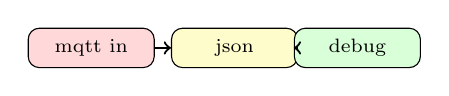
\begin{tikzpicture}[
            scale=0.65,
            every node/.style={font=\scriptsize},
            nd/.style={draw, rounded corners, minimum width=1.6cm, minimum height=0.5cm},
        ]
            \node[nd, fill=red!15] (mqtt) at (0,0) {mqtt in};
            \node[nd, fill=yellow!20] (json) at (2.8,0) {json};
            \node[nd, fill=green!15] (debug) at (5.2,0) {debug};
            \draw[->,thick] (mqtt) -- (json);
            \draw[->,thick] (json) -- (debug);
        \end{tikzpicture}

        \vspace{0.3cm}
        \fcolorbox{warnborder}{warnbg}{
        \begin{minipage}{0.9\textwidth}
            \vspace{0.05cm}
            \tiny
            \textbf{Why parse?} Node-RED receives MQTT payloads as raw strings. To access \texttt{.temp} or \texttt{.hum}, we need a JavaScript object. The json node does this conversion automatically.
            \vspace{0.05cm}
        \end{minipage}
        }
    \end{columns}
\end{frame}

\begin{frame}[fragile,shrink=5]{Exercise 2b: Extract Values + Gauges (10 min)}
    \textbf{Extract individual sensor values and display them as gauges.}

    \vspace{0.15cm}
    \begin{columns}
        \column{0.55\textwidth}
        \textbf{Function node to extract temperature:}
        \begin{lstlisting}[language=Java,basicstyle=\ttfamily\small]
msg.payload = msg.payload.temp;
return msg;
        \end{lstlisting}

        \vspace{0.1cm}
        \textbf{Steps:}
        \begin{enumerate}
            \item Add \textbf{function} node after json $\rightarrow$ extract \texttt{.temp}
            \item Connect to \textbf{ui-gauge} (Dashboard 2.0 section):
            \begin{itemize}
                \item Create Group: ``Temperature''
                \item Create Page: ``Sensors''
                \item Range: 0 to 50, Units: \textdegree{}C
            \end{itemize}
            \item \textbf{Your turn:} add a second branch for humidity
            \begin{itemize}
                \item Another function: \texttt{msg.payload.hum}
                \item Another ui-gauge: range 0--100, units \%
            \end{itemize}
            \item Deploy $\rightarrow$ open \url{http://localhost:1880/dashboard}
        \end{enumerate}

        \column{0.45\textwidth}
        \textbf{Flow with two branches:}

        \vspace{0.1cm}
        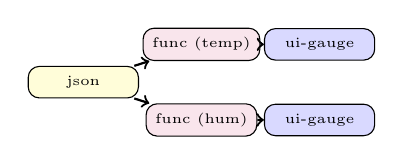
\begin{tikzpicture}[
            scale=0.6,
            every node/.style={font=\tiny},
            nd/.style={draw, rounded corners, minimum width=1.4cm, minimum height=0.4cm},
        ]
            \node[nd, fill=yellow!15] (json) at (0,0) {json};
            \node[nd, fill=purple!10] (ft) at (2.5,0.8) {func (temp)};
            \node[nd, fill=purple!10] (fh) at (2.5,-0.8) {func (hum)};
            \node[nd, fill=blue!15] (g1) at (5,0.8) {ui-gauge};
            \node[nd, fill=blue!15] (g2) at (5,-0.8) {ui-gauge};
            \draw[->,thick] (json) -- (ft);
            \draw[->,thick] (json) -- (fh);
            \draw[->,thick] (ft) -- (g1);
            \draw[->,thick] (fh) -- (g2);
        \end{tikzpicture}

        \vspace{0.2cm}
        \fcolorbox{stepborder}{stepbg}{
        \begin{minipage}{0.9\textwidth}
            \vspace{0.1cm}
            \scriptsize
            \textbf{Dashboard 2.0 hierarchy:}\\
            Base $\rightarrow$ Page $\rightarrow$ Group $\rightarrow$ Widget\\[4pt]
            First widget auto-creates all levels. Set meaningful names.
            \vspace{0.1cm}
        \end{minipage}
        }

        \vspace{0.1cm}
        \fcolorbox{warnborder}{warnbg}{
        \begin{minipage}{0.9\textwidth}
            \vspace{0.05cm}
            \tiny
            \textbf{Gauge range matters:} Indoor temp? 0--50. Freezer? $-30$ to 5. Greenhouse? 10--45. Your deployment context sets the range.
            \vspace{0.05cm}
        \end{minipage}
        }
    \end{columns}
\end{frame}

\begin{frame}[fragile,shrink=5]{Exercise 2c: Time-Series Chart + Full Pipeline (5 min)}
    \textbf{Add historical view and verify the end-to-end pipeline.}

    \vspace{0.15cm}
    \begin{columns}
        \column{0.5\textwidth}
        \textbf{Add a chart:}
        \begin{enumerate}
            \item Drag \textbf{ui-chart} from Dashboard 2.0 palette
            \item Connect to temperature function output (parallel to gauge)
            \item Create Group: ``History''
            \item Chart type: Line, X-axis: time
            \item Deploy
        \end{enumerate}

        \vspace{0.15cm}
        \textbf{Complete flow so far:}

        \vspace{0.1cm}
        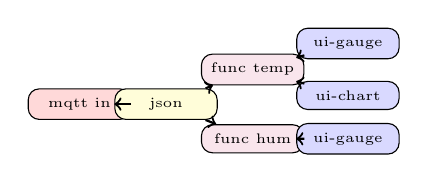
\begin{tikzpicture}[
            scale=0.55,
            every node/.style={font=\tiny},
            nd/.style={draw, rounded corners, minimum width=1.3cm, minimum height=0.35cm},
        ]
            \node[nd, fill=red!15] (mqtt) at (0,0) {mqtt in};
            \node[nd, fill=yellow!15] (json) at (2,0) {json};
            \node[nd, fill=purple!10] (ft) at (4,0.8) {func temp};
            \node[nd, fill=purple!10] (fh) at (4,-0.8) {func hum};
            \node[nd, fill=blue!15] (g1) at (6.2,1.4) {ui-gauge};
            \node[nd, fill=blue!15] (ch) at (6.2,0.2) {ui-chart};
            \node[nd, fill=blue!15] (g2) at (6.2,-0.8) {ui-gauge};
            \draw[->,thick] (mqtt) -- (json);
            \draw[->,thick] (json) -- (ft);
            \draw[->,thick] (json) -- (fh);
            \draw[->,thick] (ft) -- (g1);
            \draw[->,thick] (ft) -- (ch);
            \draw[->,thick] (fh) -- (g2);
        \end{tikzpicture}

        \column{0.5\textwidth}
        \fcolorbox{stepborder}{stepbg}{
        \begin{minipage}{0.95\textwidth}
            \vspace{0.1cm}
            \small
            \textbf{What we have now:}
            \begin{itemize}
                \item ESP32 $\rightarrow$ MQTT $\rightarrow$ Node-RED
                \item Real-time temperature gauge
                \item Real-time humidity gauge
                \item Historical line chart
                \item All at \texttt{localhost:1880/dashboard}
            \end{itemize}

            \vspace{0.1cm}
            This is a functional MVP dashboard.
            \vspace{0.1cm}
        \end{minipage}
        }

        \vspace{0.15cm}
        \fcolorbox{aiborder}{aibg}{
        \begin{minipage}{0.95\textwidth}
            \vspace{0.05cm}
            \tiny
            \textbf{Reflect:} No backend code. No cloud account. No database setup. The full sensor-to-screen pipeline runs on your laptop. When hardware arrives Saturday, only the device layer changes.
            \vspace{0.05cm}
        \end{minipage}
        }
    \end{columns}
\end{frame}

%==============================================================================
\section{Exercise 3: Alerts + Logic}
%==============================================================================

\begin{frame}[fragile,shrink=5]{Exercise 3a: Threshold Logic (10 min)}
    \textbf{Add conditional routing: alert when temperature exceeds 30\textdegree{}C.}

    \vspace{0.15cm}
    \begin{columns}
        \column{0.55\textwidth}
        \textbf{Flow:}

        \vspace{0.1cm}
        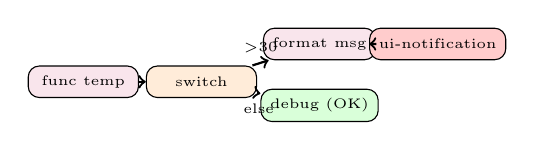
\begin{tikzpicture}[
            scale=0.6,
            every node/.style={font=\tiny},
            nd/.style={draw, rounded corners, minimum width=1.4cm, minimum height=0.4cm},
        ]
            \node[nd, fill=purple!10] (func) at (0,0) {func temp};
            \node[nd, fill=orange!15] (sw) at (2.5,0) {switch};
            \node[nd, fill=purple!10] (fmt) at (5,0.8) {format msg};
            \node[nd, fill=red!20] (notif) at (7.5,0.8) {ui-notification};
            \node[nd, fill=green!15] (ok) at (5,-0.5) {debug (OK)};
            \draw[->,thick] (func) -- (sw);
            \draw[->,thick] (sw) -- node[above,font=\tiny]{$>$30} (fmt);
            \draw[->,thick] (fmt) -- (notif);
            \draw[->,thick] (sw) -- node[below,font=\tiny]{else} (ok);
        \end{tikzpicture}

        \vspace{0.15cm}
        \textbf{Steps:}
        \begin{enumerate}
            \item Wire \textbf{switch} node after temperature function
            \item Configure two rules:
            \begin{itemize}
                \item Rule 1: \texttt{msg.payload} $>$ 30 $\rightarrow$ output 1
                \item Rule 2: otherwise $\rightarrow$ output 2
            \end{itemize}
            \item Output 1: \textbf{function} to format alert message:
            \begin{lstlisting}[language=Java,basicstyle=\ttfamily\tiny]
msg.payload = "ALERT: Temp " + msg.payload + "C exceeds 30C!";
return msg;
            \end{lstlisting}
            \item Connect to \textbf{ui-notification} (Dashboard 2.0)
            \item Output 2: connect \textbf{debug} node (normal readings)
        \end{enumerate}

        \column{0.45\textwidth}
        \fcolorbox{stepborder}{stepbg}{
        \begin{minipage}{0.9\textwidth}
            \vspace{0.1cm}
            \small
            \textbf{The switch node:}

            \vspace{0.1cm}
            Conditional routing in Node-RED.\\
            Evaluates \texttt{msg.payload} against rules.\\
            Each rule maps to a separate output wire.

            \vspace{0.1cm}
            This is the core of automation logic: \textit{if condition, then action}.
            \vspace{0.1cm}
        \end{minipage}
        }

        \vspace{0.15cm}
        \fcolorbox{warnborder}{warnbg}{
        \begin{minipage}{0.9\textwidth}
            \vspace{0.05cm}
            \tiny
            \textbf{Test it:} In Wokwi, click DHT22 and set temp $>$ 30. In the Python simulator, modify the range. Check that a notification pops up on \texttt{/dashboard}.
            \vspace{0.05cm}
        \end{minipage}
        }
    \end{columns}
\end{frame}

\begin{frame}[shrink=5]{Exercise 3b: Adapt to Your Project (5 min)}
    \textbf{Replace the generic threshold with your PES requirement.}

    \vspace{0.15cm}
    \begin{columns}
        \column{0.55\textwidth}
        \textbf{Project-specific thresholds:}

        \vspace{0.1cm}
        \begin{tabular}{lll}
            \toprule
            \textbf{Domain} & \textbf{Parameter} & \textbf{Threshold} \\
            \midrule
            Agriculture & Soil moisture & $<$ 20\% \\
            Cold chain & Temperature & Outside 2--8\textdegree{}C \\
            Structural & Vibration & $>$ 2g \\
            Indoor air & CO2 & $>$ 1000 ppm \\
            Server room & Temperature & $>$ 27\textdegree{}C \\
            Greenhouse & Humidity & $>$ 85\% \\
            \bottomrule
        \end{tabular}

        \vspace{0.15cm}
        \textbf{Your task:}
        \begin{enumerate}
            \item Change the switch threshold to match your PES
            \item Update the alert message text
            \item \textit{Optional:} add a second threshold (warning vs critical)
        \end{enumerate}

        \column{0.45\textwidth}
        \begin{block}{Engineering Value}
            \small
            Threshold logic = your PES implemented as code.\\[4pt]
            In your final report:\\
            \textit{``Threshold alerting was implemented using Node-RED flow logic at the PES-defined limit of [X].''}
        \end{block}

        \vspace{0.15cm}
        \fcolorbox{aiborder}{aibg}{
        \begin{minipage}{0.9\textwidth}
            \vspace{0.05cm}
            \tiny
            \textbf{Context matters:} AI does not know what 30\textdegree{}C means for YOUR system. Is it an HVAC threshold? A greenhouse warning? A server room emergency? You define the threshold because you understand the deployment context.
            \vspace{0.05cm}
        \end{minipage}
        }
    \end{columns}
\end{frame}

%==============================================================================
\section{Summary}
%==============================================================================

\begin{frame}[shrink=15]{What We Built Today: Full Architecture}
    \begin{center}
    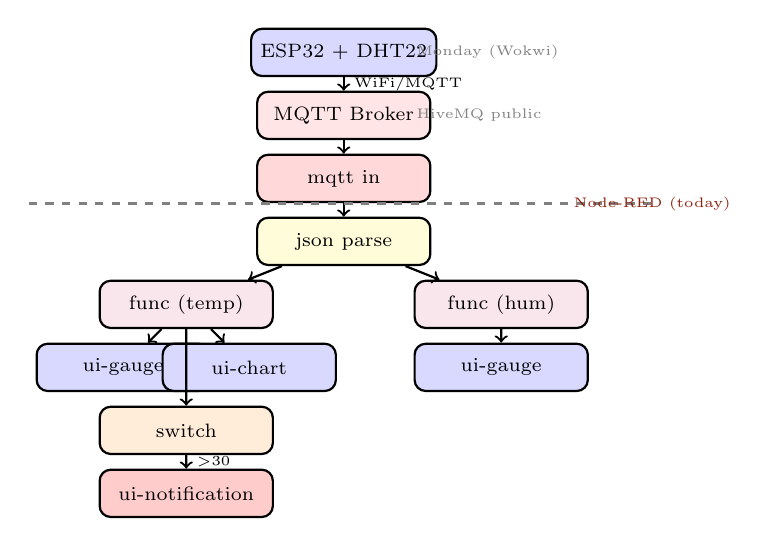
\begin{tikzpicture}[
        scale=0.8,
        every node/.style={font=\scriptsize},
        box/.style={draw, rounded corners, minimum width=2.2cm, minimum height=0.6cm, thick},
    ]
        \node[box, fill=blue!15] (esp) at (0,4) {ESP32 + DHT22};
        \node[box, fill=red!10] (broker) at (0,3) {MQTT Broker};
        \node[box, fill=red!15] (mqttin) at (0,2) {mqtt in};
        \node[box, fill=yellow!15] (json) at (0,1) {json parse};
        \node[box, fill=purple!10] (ft) at (-2.5,0) {func (temp)};
        \node[box, fill=purple!10] (fh) at (2.5,0) {func (hum)};
        \node[box, fill=blue!15] (g1) at (-3.5,-1) {ui-gauge};
        \node[box, fill=blue!15] (ch) at (-1.5,-1) {ui-chart};
        \node[box, fill=orange!15] (sw) at (-2.5,-2) {switch};
        \node[box, fill=red!20] (notif) at (-2.5,-3) {ui-notification};
        \node[box, fill=blue!15] (g2) at (2.5,-1) {ui-gauge};

        \draw[->,thick] (esp) -- node[right,font=\tiny]{WiFi/MQTT} (broker);
        \draw[->,thick] (broker) -- (mqttin);
        \draw[->,thick] (mqttin) -- (json);
        \draw[->,thick] (json) -- (ft);
        \draw[->,thick] (json) -- (fh);
        \draw[->,thick] (ft) -- (g1);
        \draw[->,thick] (ft) -- (ch);
        \draw[->,thick] (ft) -- (sw);
        \draw[->,thick] (sw) -- node[right,font=\tiny]{$>$30} (notif);
        \draw[->,thick] (fh) -- (g2);

        % Labels
        \node[font=\tiny, text=gray, right] at (1,4) {Monday (Wokwi)};
        \node[font=\tiny, text=gray, right] at (1,3) {HiveMQ public};

        \draw[dashed, gray, thick] (-5,1.6) -- (5,1.6);
        \node[font=\tiny, text=nodered, right] at (3.5,1.6) {Node-RED (today)};
    \end{tikzpicture}
    \end{center}

    \vspace{0.1cm}
    \begin{columns}
        \column{0.33\textwidth}
        \centering
        \textbf{Exercise 1}\\
        {\small MQTT $\rightarrow$ Debug}\\
        {\tiny Receive + verify data}

        \column{0.33\textwidth}
        \centering
        \textbf{Exercise 2}\\
        {\small Parse $\rightarrow$ Gauges + Chart}\\
        {\tiny Visualize in real time}

        \column{0.33\textwidth}
        \centering
        \textbf{Exercise 3}\\
        {\small Switch $\rightarrow$ Notification}\\
        {\tiny Automate with thresholds}
    \end{columns}
\end{frame}

%==============================================================================
\section{Wrap-Up}
%==============================================================================

\begin{frame}[shrink=10]{Common Issues + Debugging Tips}
    \begin{columns}
        \column{0.5\textwidth}
        \textbf{Installation:}
        \begin{itemize}
            \item \textbf{Node-RED won't start:} check \texttt{node --version} $\geq$ 18
            \item \textbf{Permission errors (Mac):}\\
                  \texttt{sudo npm install -g --unsafe-perm node-red}
            \item \textbf{Dashboard nodes missing:}\\
                  Menu $\rightarrow$ Manage Palette $\rightarrow$ Install\\
                  Search: \texttt{@flowfuse/node-red-dashboard}\\
                  {\tiny (Not the deprecated \texttt{node-red-dashboard})}
        \end{itemize}

        \vspace{0.15cm}
        \textbf{MQTT:}
        \begin{itemize}
            \item \textbf{``Disconnected'':} verify broker config\\
                  \texttt{broker.hivemq.com} port \texttt{1883}\\
                  No username, no password, no TLS
            \item \textbf{No data arriving:} check topic spelling matches exactly what the ESP32/simulator publishes
        \end{itemize}

        \column{0.5\textwidth}
        \textbf{Dashboard:}
        \begin{itemize}
            \item \textbf{Blank page at /dashboard:}\\
                  Verify Group + Page created in widget config
            \item \textbf{Gauges show nothing:}\\
                  Check debug panel first; data must flow
        \end{itemize}

        \vspace{0.15cm}
        \textbf{Function nodes:}
        \begin{itemize}
            \item \textbf{Most common mistake:}

            \vspace{0.05cm}
            \fcolorbox{warnborder}{warnbg}{
            \begin{minipage}{0.85\textwidth}
                \centering\small
                Forgetting \texttt{return msg;} at the end.\\
                Without it, the message stops and nothing downstream receives data.
            \end{minipage}
            }
        \end{itemize}

        \vspace{0.15cm}
        \textbf{General debugging strategy:}
        \begin{enumerate}
            \item Add \textbf{debug} nodes after each step
            \item Deploy after every change
            \item Work left to right: verify each node
        \end{enumerate}
    \end{columns}
\end{frame}

\begin{frame}{Deliverables + Next Steps}
    \textbf{Before you leave today:}

    \vspace{0.2cm}
    \begin{enumerate}
        \item \textbf{Export your Node-RED flow:} Menu $\rightarrow$ Export $\rightarrow$ Clipboard $\rightarrow$ save as \texttt{.json}
        \item \textbf{Screenshot your dashboard:} with live data
        \item \textbf{Post both} on Canvas discussion board
    \end{enumerate}

    \vspace{0.3cm}
    \textbf{What you've built this week so far:}

    \vspace{0.15cm}
    \begin{tabular}{lll}
        \toprule
        \textbf{Session} & \textbf{What you built} & \textbf{Status} \\
        \midrule
        Mon 23 & ESP32 firmware + MQTT publish & \checkmark Done \\
        \textbf{Today (Wed 25)} & \textbf{Node-RED flows + dashboard} & \textbf{\checkmark Done} \\
        Thu 26 & IoT dataset analysis & Tomorrow \\
        \midrule
        Mon 30+ & Real hardware in lab & Firmware ready \\
        \bottomrule
    \end{tabular}

    \vspace{0.3cm}
    \fcolorbox{stepborder}{stepbg}{
    \begin{minipage}{0.95\textwidth}
        \small
        \textbf{Portfolio:} Your Node-RED flow JSON + dashboard screenshot = evidence of ``IoT data pipeline design and automation logic.''
    \end{minipage}
    }
\end{frame}

\end{document}
